\hypertarget{tulokset}{%
\chapter{Tulokset}\label{tulokset}}

\hypertarget{prototyyppiohjelman-esittely}{%
\section{Prototyyppiohjelman
esittely}\label{prototyyppiohjelman-esittely}}

Prototyyppiohjelma on yksinkertainen yhden sivun selainsovellus. Sen
avulla voi luoda käyntejä, laskuttaa niitä, koota laskuja
koontilaskuiksi ja hyvittää yksittäisiä laskurivejä.

Ohjelman pääkäyttöliittymä on esitetty kuvassa
\ref{rakkine_default-view}

Laskujen sisältöjä voi tarkastella, ja ohjelma laskee laskujen avoimet
summat.

Lisäksi käyttöliittymästä voi valita maksajan luotavalle laskulle.
Mikäli maksajia valitaan useampia, ohjelma jakaa käynnit kahdelle eri
maksajalle. Tämä on esitetty kuvassa \ref{rakkine_dividing}

\begin{figure}
\centering
\includegraphics[width=\textwidth,height=0.6\textheight]{illustration/screenshots/Laskurakkine.png}
\caption{\label{rakkine_default-view}Laskujen lisäysnäkymä}
\end{figure}

Erillisessä listanäkymässä (Kuva \ref{rakkine_list-view}) voi
tarkastella luotujen käyntien tilaa sekä laskutettavan myynnin tilaa.
Ohjelma näyttää, onko käynti laskutettu vai laskuttamaton. Myynnin
osalta ohjelma näyttää, miten myynti jakautuu eri maksajille, ja onko
summa avoin, laskutettu vai hyvitetty.

\begin{figure}
\centering
\includegraphics[width=\textwidth,height=0.6\textheight]{illustration/screenshots/List-view.png}
\caption{\label{rakkine_list-view}Ohjelman listanäkymä}
\end{figure}

\begin{figure}
\centering
\includegraphics[width=\textwidth,height=0.6\textheight]{illustration/screenshots/credited.png}
\caption{\label{rakkine_credited}Ohjelma näyttää, että yksittäinen
laskurivi on hyvitetty}
\end{figure}

Kuvassa \ref{rakkine_credited} on esitetty miten ohjelma näyttää
hyvitetyn laskurivin.

\begin{figure}
\centering
\includegraphics[width=\textwidth,height=0.6\textheight]{illustration/screenshots/Dividing.png}
\caption{\label{rakkine_dividing}Esimerkki käynnin jakamiesta usealle
maksajalle}
\end{figure}

Käytin asiakasohjelman tekemiseen niin vähän aikaa kuin mahdollista. Se
näkyy tyylin hiomattomuutena. Luonnosmaisen näköinen ulkoasu myös
kommunikoi muille prosessiin osallistuville, että ohjelmisto tai
etenkään sen käyttöliittymä ei ole tarkoitettu tuotantokäyttöön, vaan
apuvälineeksi erilaisten tietomallin piirteiden kartoittamiseen.

\hypertarget{kuvaus-tyuxf6mallista}{%
\section{Kuvaus työmallista}\label{kuvaus-tyuxf6mallista}}

Seuraavaksi kuvaan lyhyesti ne periaatteet, joiden varaan tämä työmalli
rakentuu.

\hypertarget{lyhyet-iteraatiot}{%
\subsection{Lyhyet iteraatiot}\label{lyhyet-iteraatiot}}

Lyhyet iteraatiot, joiden välissä pidetään suunnittelutapaaminen, ovat
ehdoton edellytys mallin ripeälle kehittämiselle. On tärkeää, että
iteraation kuluessa syntyy käyttökelpoinen ohjelmistoversio, jonka
avulla mallin toimivuutta voidaan testata ja todentaa.

\hypertarget{keskusteleva-suhde-tuoteomistajan-ja-kehittuxe4juxe4n-vuxe4lilluxe4}{%
\subsection{Keskusteleva suhde tuoteomistajan ja kehittäjän
välillä}\label{keskusteleva-suhde-tuoteomistajan-ja-kehittuxe4juxe4n-vuxe4lilluxe4}}

Koska tavoitteena on luoda kieli, jota voivat käyttää niin ohjelmoijat
kuin liiketoimintaväkikin, sen kehittämiseen luontevin ja
todennäköisesti ainoa tapa on rakentaa mallia keskustelevalla otteella.

\hypertarget{kuxe4yttuxe4juxe4tarinoihin-pohjautuva-tyuxf6lista}{%
\subsection{Käyttäjätarinoihin pohjautuva
työlista}\label{kuxe4yttuxe4juxe4tarinoihin-pohjautuva-tyuxf6lista}}

Ketterän kehityksen työkalupakista peräisin oleva ajatus
yksinkertaisista käyttäjätarinoista soveltuu hyvin tietomallin
kehittämisen lähtökohdaksi. Kun huomion keskipisteenä ovat ne asiat,
joita käyttäjä voi ohjelmistolla tehdä, on myös syntyvä malli lähempänä
alan realismia.

\hypertarget{rajapintaskeeman-rakentaminen-kuxe4sitteiden-pohjalta}{%
\subsection{Rajapintaskeeman rakentaminen käsitteiden
pohjalta}\label{rajapintaskeeman-rakentaminen-kuxe4sitteiden-pohjalta}}

GraphQL-rajapintaskeema kannattaa rakentaa ennenkuin kirjoittaa skeeman
toteuttavaa koodia. Näin kielen käsitteet ja niiden väliset suhteet
tulevat formaalisti ilmaistuksi. Ohjelmakoodin kirjoittamisen aikana
skeema saattaa myös tarkentua, ja silloin kannattaa muutokset tehdä
välittömästi.

\hypertarget{koodin-ja-mallin-pituxe4minen-luxe4hekkuxe4in}{%
\subsection{Koodin ja mallin pitäminen
lähekkäin}\label{koodin-ja-mallin-pituxe4minen-luxe4hekkuxe4in}}

Välttämätön osa tätä työtyyliä on koodin ja mallin vastaavuus. Mallissa
käytettävät käsitteet on löydyttävä koodista, ja koodissa tulisi olla
lähinnä vain nämä käsitteet ja niiden väliset suhteet sellaisina, kuin
ne \glslink{ubilang}{kaikenkattavassa kielessä} ilmenevät.

\hypertarget{voimakkaat-refaktoroinnit}{%
\subsection{Voimakkaat refaktoroinnit}\label{voimakkaat-refaktoroinnit}}

Voimakkaat refaktoroinnit ovat keino muokata koodin esittämästä mallista
joustava ja ilmaisuvoimainen. Nämä refaktoroinnit vaativat ehdottomasti
tuekseen jämerän yksikkötestisetin. Sen rakentaminen onnistuu
käytännössä vain testit edellä tekemällä.

\hypertarget{ohjelmoinnissa-vastaan-tulleet-ongelmat-jatkosuunnittelun-luxe4htuxf6kohtina}{%
\subsection{Ohjelmoinnissa vastaan tulleet ongelmat jatkosuunnittelun
lähtökohtina}\label{ohjelmoinnissa-vastaan-tulleet-ongelmat-jatkosuunnittelun-luxe4htuxf6kohtina}}

Suunnittelutapaamisten ja ohjelmointiprosessin välinen yhteys ei saa
olla vain yksisuuntainen. Mikäli suunnittelutapaaminen nähdään ainoana
osana prosessia, jossa suunnittelua tapahtuu ja ohjelmointi pelkästään
suunnitelmien mekaanisena toteuttamisena, hyödyt tästä
työskentelytyylistä jäävät hyvin vähäisiksi. Ohjelmointiprosessi on
suunnittelutyön toisenlainen vaihe, ja siinä ilmenevät ongelmat ovat
oivallinen maaperä seuraavan suunnittelutapaamisen aiheiksi.

\hypertarget{tyuxf6mallin-haasteita}{%
\section{Työmallin haasteita}\label{tyuxf6mallin-haasteita}}

Tämä työmalli vaatii ohjelmoijalta paljon. Se edellyttää jatkuvaa
kiinnostusta sovellusalueen piirteistä, ja laajaa tarkkaavuutta
suunnittelutapaamisten keskuisteluissa. Lisäksi se edellyttää kykyä
sietää epävarmuutta ja muuttaa suunnitelmia usein ja isosti. Teknisellä
tasolla työmalli edellyttää kykyä joustavan ohjelmiston
suunnittelemiseen, laajojen refaktorointien tekemiseen kireässä
aikataulussa pysyen ja tiukkaa keskittymistä niihin päämääriin, jotka
mallin kehittämisessä on kulloinkin asetettu.

Jotta tällainen työmalli voi olla hedelmällinen tuotantotasoisen
ohjelmiston tekemisessä, se edellyttää myös, että työtyyli ohjelmoijan
ympärillä vastaa tällaista tekemisen tapaa. Liiketoimintavetoisella
suunnittelulla on vaikutuksia paitsi ohjelmistotuotannon prosessiin,
myös sitä ympäröiviin prosesseihin, kuten asiakastarpeiden kokoamiseen
ja tulevan kehitystyön suunnittelemiseen.

\hypertarget{parannuksia-tietomalliin}{%
\section{Parannuksia tietomalliin}\label{parannuksia-tietomalliin}}

Viiden viikon aikana syntyi pieni malli laskutukseen tietorakenteen
parantamiseksi. Lisäksi löytyi kaksi pientä ideaa, joita voi hyödyntää,
kun ohjelmistoa kehitetään.

Pieni malli laskutuksen parantamiseksi on esitetty kuvassa
\ref{finalmodel1-again}. Se pitää sisällään ajatuksen käynnin
muuttumisesta myynniksi, kun se saapuu laskutuksen piiriin. Oma
erikoisuutensa on myös käynnin jakamiseen liittyvä jakoperuste - tätä ei
ohjelmistoon toteutettu, mutta suunnitteluvaiheessa se tuntui
hyödylliseltä idealta.

\begin{figure}
\centering
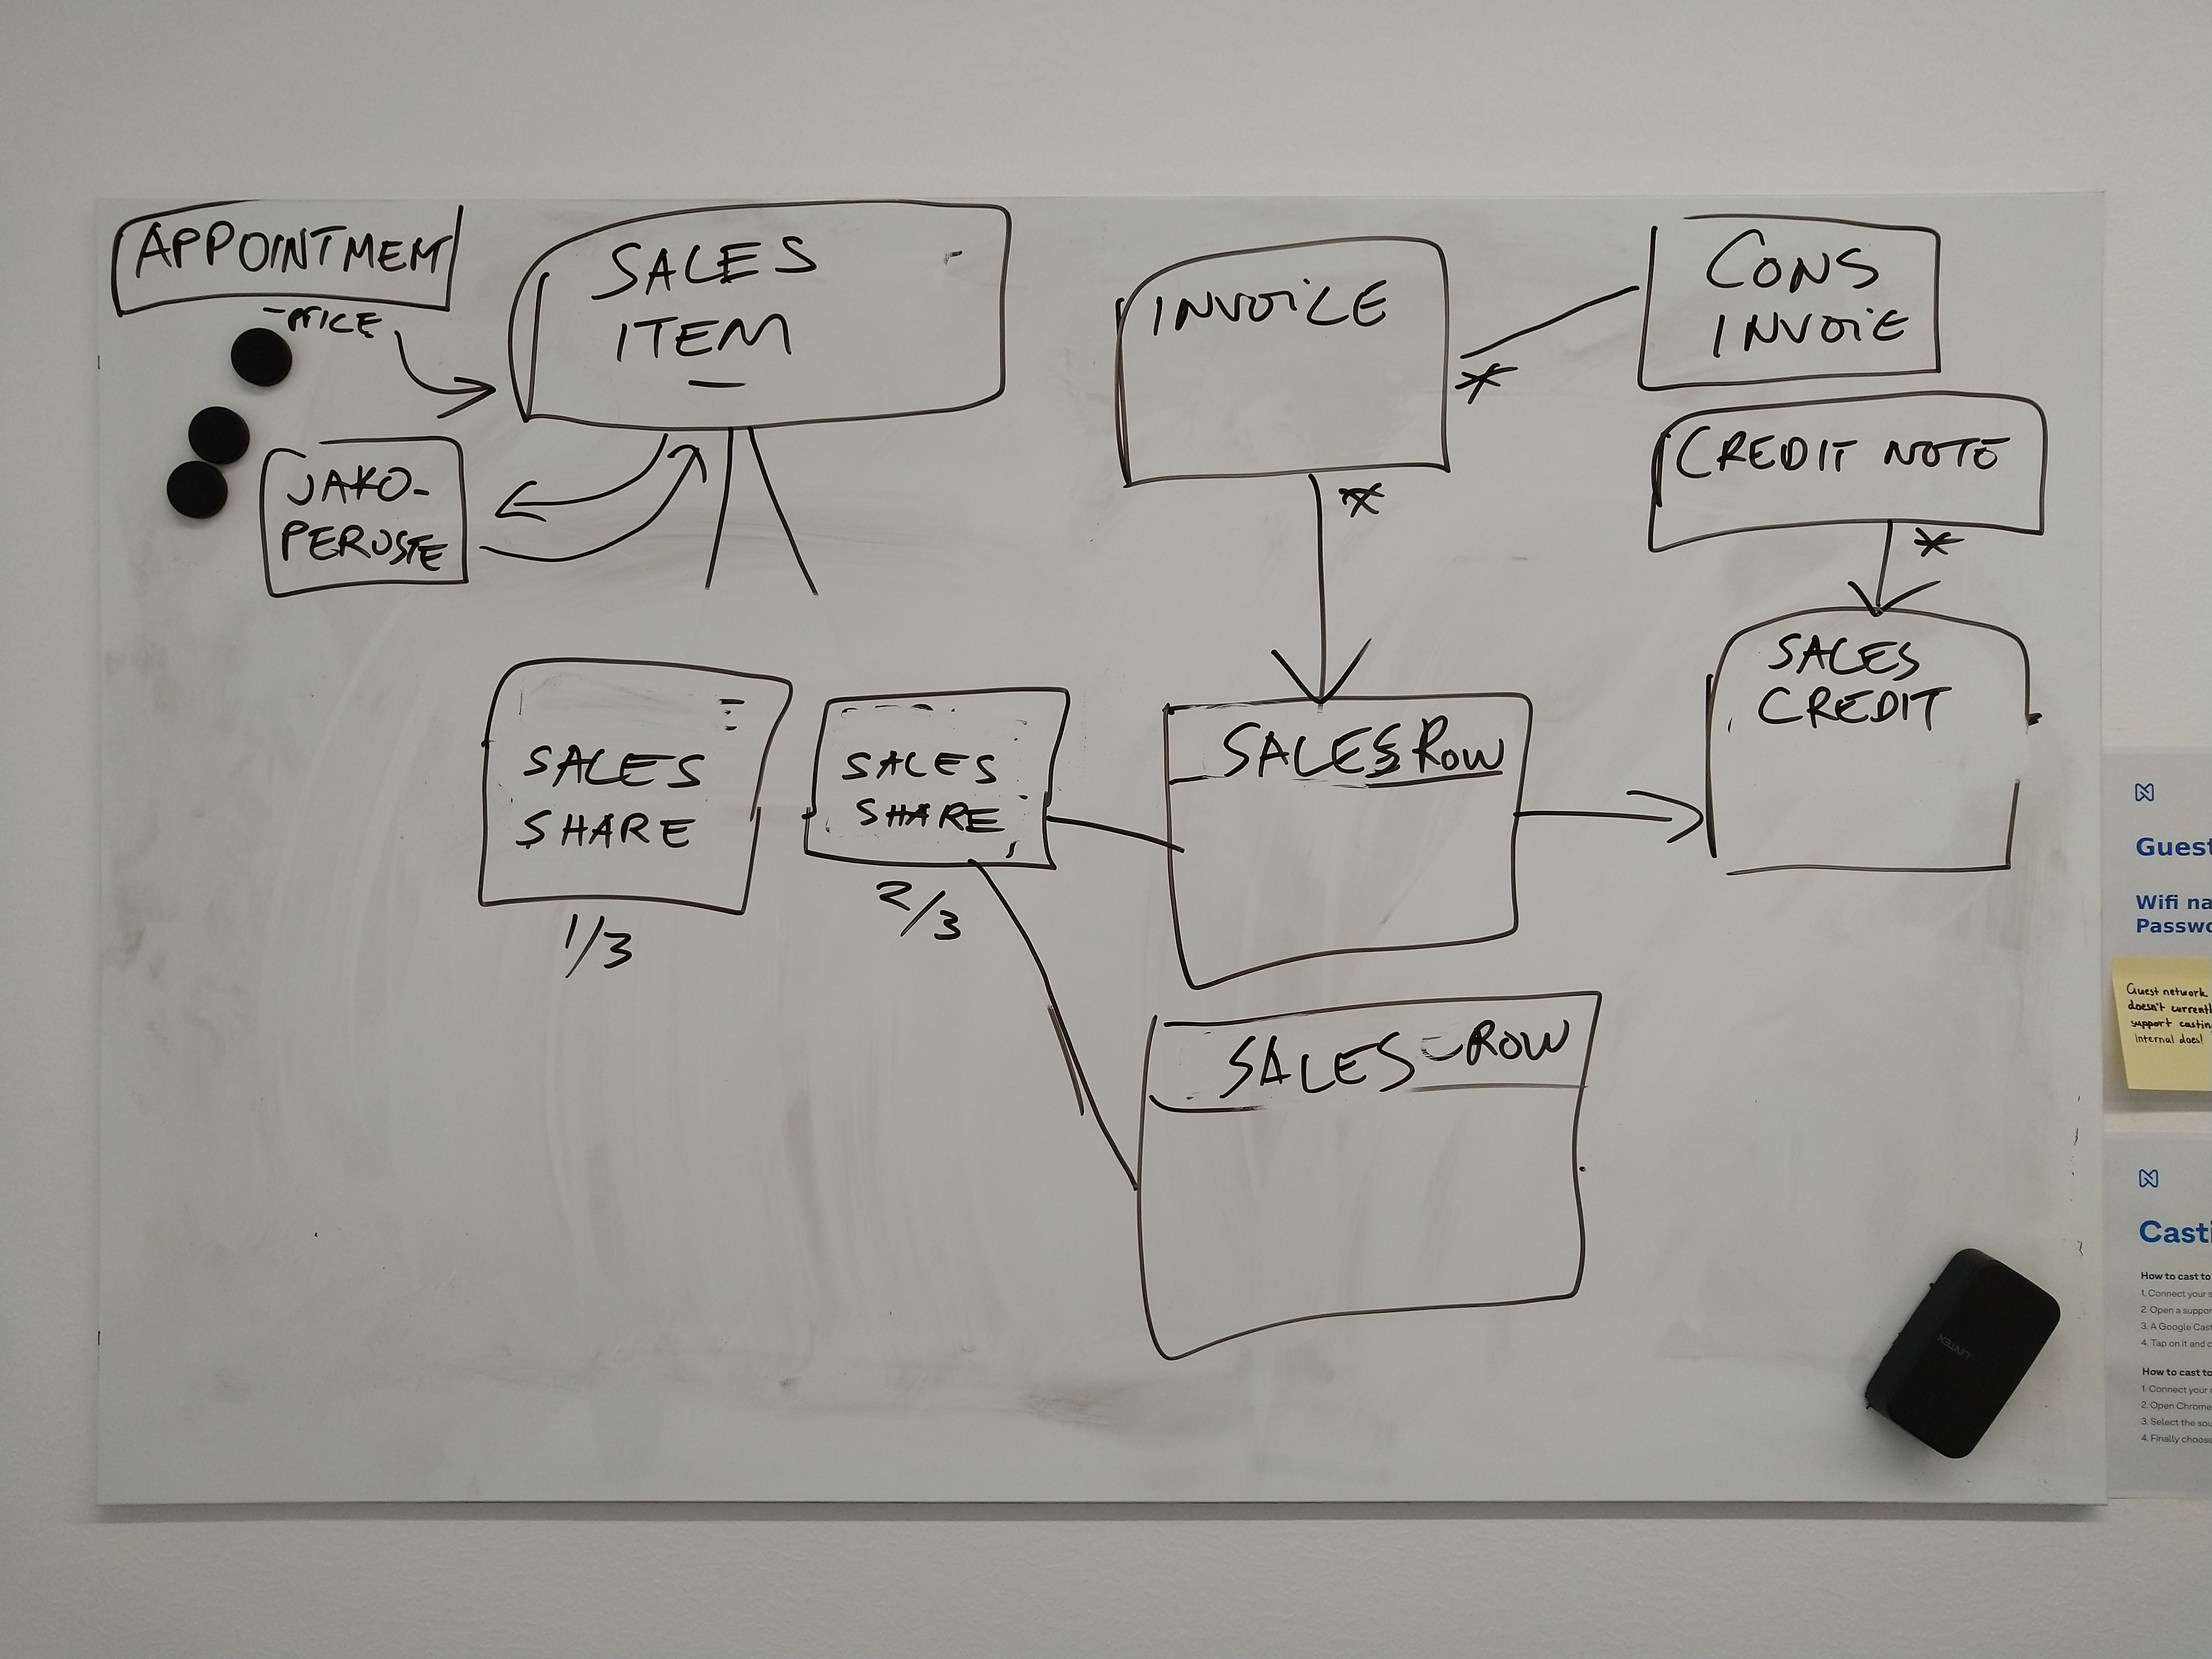
\includegraphics[width=\textwidth,height=0.3\textheight]{illustration/malli4.jpg}
\caption{\label{finalmodel1-again}Lopullinen malli}
\end{figure}

Kaksi pientä ideaa ovat molemmat käyttökelpoisia erillään mallista.
Ensimmäinen niistä on myynnin, myyntirivin ja hyvitysrivin välinen
tiivis yhteysketju. Tämä idea (kuva \ref{finalidea1})mahdollistaa hyvin
yksinkertaisen ja joustavan myynnin laskutus- ja hyvityslogiikan.

\begin{figure}
\centering
\includegraphics[width=\textwidth,height=0.3\textheight]{illustration/final-idea-1.jpg}
\caption{\label{finalidea1}Idea 1}
\end{figure}

Toinen pieni idea on, että käynti kannattaisi erottaa selkeästi laskulle
tulevasta myynnistä. Tällöin on mahdollista myös esimerkiksi vaihtaa
myöhemmin maksajaa, jolta käynti laskutetaan, ilman että jo
muodostettuihin laskuihin tarvitsee kajota. Tämä ajatus on esitetty
kuvassa \ref{finalidea2}.

\begin{figure}
\centering
\includegraphics[width=\textwidth,height=0.3\textheight]{illustration/final-idea-2.jpg}
\caption{\label{finalidea2}Idea 2}
\end{figure}
